\chapter{THIẾT KẾ KHÁI QUÁT}
    \section{Thiết kế khái quát cơ khí}

        \subsection{Mục tiêu thiết kế cơ khí}

            \hspace{0.5cm} Mục tiêu của phần thiết kế cơ khí là xây dựng mô hình robot nhện 6 chân có khả năng di chuyển ổn định, kết cấu gọn nhẹ, dễ chế tạo và phù hợp với điều kiện thực nghiệm. Robot được thiết kế theo hướng cân bằng giữa độ ổn định, khả năng cơ động, độ phức tạp điều khiển và chi phí chế tạo.

            \hspace{0.5cm} Các yêu cầu thiết kế cơ bản của robot được xác định như sau:

            \begin{itemize}
                \item Robot có cấu trúc dạng hexapod với 6 chân bố trí đối xứng hai bên thân.
                \item Mỗi chân có 3 bậc tự do, cho phép thực hiện chuyển động tiến/lùi, nâng/hạ chân và điều chỉnh vị trí tiếp xúc với mặt đất.
                \item Khối lượng toàn bộ robot dự kiến khoảng 2 kg.
                \item Vận tốc di chuyển mong muốn của robot là 5 cm/s.
                \item Kết cấu cơ khí phải đủ cứng vững, hạn chế biến dạng trong quá trình robot di chuyển.
                \item Các cụm cơ khí cần thuận tiện cho quá trình lắp ráp, tháo rời, kiểm tra và bảo trì.
            \end{itemize}

        \subsection{Lựa chọn cấu hình robot}

            \hspace{0.5cm} Robot di chuyển bằng chân có thể được thiết kế theo nhiều cấu hình khác nhau, phổ biến là 4 chân, 6 chân hoặc 8 chân. Mỗi cấu hình có ưu và nhược điểm riêng về độ ổn định, số lượng cơ cấu truyền động, độ phức tạp điều khiển và chi phí chế tạo.

            \hspace{0.5cm} Cấu hình 4 chân có ưu điểm là đơn giản và sử dụng ít động cơ, tuy nhiên khả năng ổn định tĩnh hạn chế hơn khi robot nhấc chân để di chuyển. Cấu hình 8 chân cho độ ổn định cao nhưng làm tăng số lượng động cơ, khối lượng, chi phí và độ phức tạp điều khiển. Vì vậy, trong phạm vi đề tài, cấu hình 6 chân được lựa chọn vì đảm bảo sự cân bằng hợp lý giữa độ ổn định, tính cơ động và khả năng chế tạo.

            \hspace{0.5cm} Các dáng đi phổ biến của robot hexapod bao gồm:

            \begin{itemize}
                \item \textbf{Tripod gait}: 3 chân nhấc lên và 3 chân còn lại chống xuống đất. Robot chia 6 chân thành hai nhóm, mỗi nhóm gồm 3 chân. Trong một nửa chu kỳ, một nhóm 3 chân tiếp xúc với mặt đất để chống đỡ thân robot, trong khi nhóm còn lại được nhấc lên và đưa về phía trước. Ưu điểm là tốc độ di chuyển tương đối tốt, chu kỳ bước đơn giản và thuận lợi cho việc lập trình điều khiển.
                \item \textbf{Quadruped gait}: 4 chân chống và 2 chân di chuyển. Dáng đi này có độ ổn định cao hơn tripod gait nhưng tốc độ di chuyển thường thấp hơn và quá trình phối hợp chuyển động giữa các chân phức tạp hơn.
                \item \textbf{One-by-one gait}: Từng chân một di chuyển trong khi các chân còn lại tiếp xúc với mặt đất. Dáng đi này có độ ổn định cao, phù hợp với robot di chuyển chậm hoặc cần vượt địa hình khó, tuy nhiên tốc độ di chuyển thấp.
            \end{itemize}

            \hspace{0.5cm} Trong phạm vi đề tài, robot được định hướng sử dụng dáng đi tripod gait do vận tốc mong muốn không quá cao nhưng vẫn cần đảm bảo khả năng di chuyển linh hoạt. Dáng đi này phù hợp với cấu hình 6 chân vì tại mỗi thời điểm vẫn có 3 chân tiếp xúc mặt đất, tạo thành vùng đỡ ổn định cho thân robot.

            \begin{table}[H]
            \centering
            \caption{So sánh sơ bộ các cấu hình robot di chuyển bằng chân}
            \begin{tabular}{|p{2cm}|p{5cm}|p{5cm}|p{3.5cm}|}
            \hline
            \textbf{Cấu hình} & \textbf{Ưu điểm} & \textbf{Nhược điểm} & \textbf{Đánh giá} \\
            \hline
            4 chân & Kết cấu đơn giản, ít động cơ & Khó ổn định khi di chuyển & Không phù hợp với yêu cầu ổn định \\
            \hline
            6 chân & Ổn định tốt, gait đa dạng, số động cơ hợp lý & Điều khiển phức tạp hơn 4 chân & Được lựa chọn \\
            \hline
            8 chân & Ổn định cao & Nhiều động cơ, chi phí và khối lượng tăng & Không cần thiết cho phạm vi đề tài \\
            \hline
            \end{tabular}
            \end{table}

            \begin{table}[H]
            \centering
            \caption{Thông số thiết kế cơ bản của robot}
            \begin{tabular}{|l|l|}
            \hline
            \textbf{Thông số} & \textbf{Giá trị lựa chọn} \\
            \hline
            Số chân & 6 \\
            \hline
            Số bậc tự do mỗi chân & 3 \\
            \hline
            Tổng số động cơ servo & 18 \\
            \hline
            Khối lượng robot & Xấp xỉ 2 kg \\
            \hline
            Vận tốc mong muốn & 5 cm/s \\
            \hline
            Cấu trúc chuyển động chính & Dáng đi tripod gait \\
            \hline
            \end{tabular}
            \end{table}

        \subsection{Cấu trúc tổng thể của robot}

            \hspace{0.5cm} Robot được chia thành hai nhóm cơ khí chính gồm thân robot và các cụm chân. Thân robot đóng vai trò là kết cấu trung tâm để gá lắp động cơ servo, mạch điều khiển, pin và các chi tiết liên kết. Các cụm chân được bố trí đối xứng hai bên thân nhằm phân bố tải trọng đều, hạn chế lệch trọng tâm và hỗ trợ robot giữ cân bằng trong quá trình di chuyển.

            \hspace{0.5cm} Mỗi bên thân robot gồm 3 chân, tương ứng với chân trước, chân giữa và chân sau. Mỗi chân có 3 khớp điều khiển bằng servo, do đó tổng số servo cần sử dụng cho toàn bộ robot là:
            \begin{equation}
                N_\text{servo} = 6 \times 3 = 18 \text{ servo}
            \end{equation}

            \hspace{0.5cm} Cách bố trí này giúp robot có khả năng thực hiện các chuyển động cơ bản như tiến, lùi, xoay trái, xoay phải và điều chỉnh tư thế thân khi cần thiết.

            \begin{figure}[H]
            \centering
            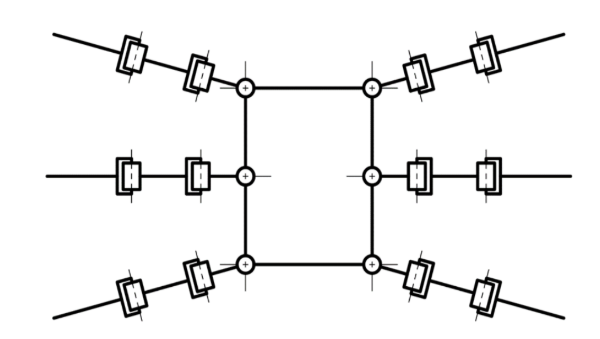
\includegraphics[width=0.85\textwidth]{pictures/hexapod_layout.png}
            \caption{Sơ đồ bố trí tổng thể robot hexapod 6 chân}
            \end{figure}

        \subsection{Cấu trúc bậc tự do của mỗi chân}

            \hspace{0.5cm} Mỗi chân robot được thiết kế với 3 bậc tự do, tương ứng với ba khớp chính là Coxa, Femur và Tibia. Cấu trúc này cho phép chân robot vừa tạo chuyển động theo phương ngang để sinh bước, vừa nâng/hạ chân và điều chỉnh điểm tiếp xúc với mặt đất.

            \begin{itemize}
                \item \textbf{Khớp Coxa}: Là khớp gần thân robot nhất, tương ứng với khớp hông. Khớp này tạo chuyển động quay theo phương ngang, giúp chân robot đưa ra phía trước hoặc phía sau trong quá trình di chuyển. Chuyển động của khớp Coxa ảnh hưởng trực tiếp đến chiều dài bước và hướng di chuyển của robot.
                \item \textbf{Khớp Femur}: Là khớp thứ hai của chân, tương ứng với khớp đùi. Khớp này có nhiệm vụ nâng hoặc hạ chân, đồng thời góp phần điều chỉnh chiều cao thân robot so với mặt đất. Đây là một trong các khớp chịu tải quan trọng do phải tạo mômen để nâng đỡ một phần trọng lượng của robot.
                \item \textbf{Khớp Tibia}: Là khớp cuối của chân, tương ứng với khớp chày. Khớp này giúp điều chỉnh vị trí tiếp xúc của chân với mặt đất, hỗ trợ robot đứng vững và thích nghi tốt hơn với sai lệch nhỏ của bề mặt di chuyển.
            \end{itemize}

            \begin{figure}[H]
            \centering
            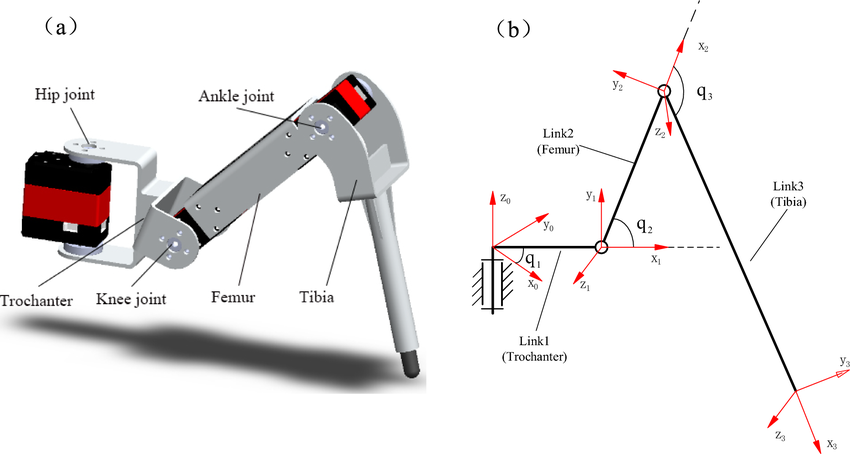
\includegraphics[width=0.7\textwidth]{pictures/leg_3dof.png}
            \caption{Mô hình 3 bậc tự do của một chân robot}
            \end{figure}

        \subsection{Định hướng bố trí cơ khí}

            \hspace{0.5cm} Về bố trí cơ khí, robot được thiết kế theo dạng đối xứng qua trục dọc thân. Mỗi bên thân gồm 3 chân, tương ứng với chân trước, chân giữa và chân sau. Cách bố trí này giúp phân bố tải trọng đều hơn, giảm sai lệch trọng tâm và tạo điều kiện thuận lợi cho robot thực hiện các dáng đi tuần hoàn.

            \hspace{0.5cm} Mạch điều khiển và pin được ưu tiên đặt gần vùng trung tâm thân robot nhằm hạn chế lệch trọng tâm. Việc bố trí khối lượng tập trung gần tâm hình học giúp robot ổn định hơn khi chuyển pha giữa các nhóm chân, đồng thời giảm mômen gây nghiêng thân khi robot di chuyển.

            \hspace{0.5cm} Các cụm chân được thiết kế dạng module, có thể tháo lắp tương đối độc lập. Cách thiết kế này giúp thuận tiện trong quá trình chế tạo, thay thế linh kiện, kiểm tra động cơ và hiệu chỉnh cơ khí.

            \hspace{0.5cm} Yêu cầu chung đối với bố trí cơ khí:
            \begin{itemize}
                \item Các chân hai bên phải được bố trí đối xứng qua trục dọc thân robot.
                \item Trọng tâm robot nên nằm gần tâm hình học của thân.
                \item Các servo phải được lắp chắc chắn để hạn chế rung lắc khi hoạt động.
                \item Các khớp chân phải chuyển động tự do, không va chạm với thân robot hoặc các chi tiết lân cận.
                \item Thân robot cần đủ cứng vững để hạn chế biến dạng khi chịu tải từ 6 cụm chân và các linh kiện lắp trên thân.
            \end{itemize}

        \subsection{Kết luận lựa chọn thiết kế khái quát}

            \hspace{0.5cm} Từ các phân tích trên, đề tài lựa chọn mô hình robot nhện 6 chân với mỗi chân gồm 3 bậc tự do. Cấu hình này cho phép robot di chuyển linh hoạt, duy trì ổn định tốt hơn so với cấu hình 4 chân, đồng thời không làm tăng quá nhiều khối lượng và chi phí như cấu hình 8 chân.

            \hspace{0.5cm} Với khối lượng robot dự kiến khoảng 2 kg và vận tốc mong muốn 4 cm/s, robot không yêu cầu tốc độ quá cao nhưng cần đảm bảo khả năng chịu tải, độ cứng vững và độ ổn định trong quá trình di chuyển. Dáng đi tripod được lựa chọn làm nguyên lý di chuyển chính do có cấu trúc điều khiển tương đối đơn giản, tốc độ di chuyển tốt và phù hợp với cấu hình robot 6 chân.

            \hspace{0.5cm} Kết quả lựa chọn thiết kế khái quát là cơ sở để thực hiện các bước thiết kế chi tiết tiếp theo, bao gồm thiết kế thân robot, thiết kế cụm chân, tính toán lựa chọn động cơ, kiểm nghiệm vận tốc và phân tích độ bền của kết cấu.

    \section{Thiết kế khái quát điện}
        \subsection{Lựa chọn phương án điện}
            \subsubsection{Phương án vi điều khiển (Microcontroller)}

            \hspace{0.5cm} Vi điều khiển là thành phần trung tâm của hệ thống điều khiển, chịu trách nhiệm tính toán thuật toán IK, điều phối gait controller, giao tiếp với các module ngoại vi và xử lý lệnh điều khiển từ xa. Nhóm đề xuất và so sánh ba phương án vi điều khiển phổ biến:

            \begin{table}[H]
            \centering
            \caption{So sánh các phương án vi điều khiển}
            \label{tab:mcu_options}
            \begin{tabular}{|>{\centering\arraybackslash}m{2.5cm}|>{\centering\arraybackslash}m{3.8cm}|>{\centering\arraybackslash}m{3.8cm}|>{\centering\arraybackslash}m{3.8cm}|}
            \hline
            \textbf{Tiêu chí} & \textbf{Arduino Mega 2560} & \textbf{STM32F103C8T6} & \textbf{ESP32} \\
            \hline
            \textbf{Xung nhịp} & 16 MHz & 72 MHz & 240 MHz (dual-core) \\
            \hline
            \textbf{RAM} & 8 KB & 20 KB & 520 KB \\
            \hline
            \textbf{WiFi / Bluetooth} & Không & Không & Tích hợp sẵn \\
            \hline
            \textbf{Giao tiếp} & UART, SPI, I\textsuperscript{2}C & UART, SPI, I\textsuperscript{2}C & UART, SPI, I\textsuperscript{2}C, CAN \\
            \hline
            \textbf{Môi trường lập trình} & Arduino IDE & STM32CubeIDE, VSCode + PlatformIO & Arduino IDE, VSCode + ESP-IDF, PlatformIO \\
            \hline
            \end{tabular}
            \end{table}

            \textbf{Kết luận:} Nhóm lựa chọn \textbf{ESP32} làm vi điều khiển trung tâm. Với xung nhịp 240 MHz dual-core và RAM 520 KB, ESP32 đủ năng lực xử lý đồng thời thuật toán IK cho 6 chân và gait controller trong thời gian thực. WiFi và Bluetooth tích hợp sẵn loại bỏ hoàn toàn nhu cầu thêm module không dây ngoài, giúp đơn giản hóa phần cứng và giảm chi phí. ESP32 cũng hỗ trợ linh hoạt nhiều môi trường lập trình (Arduino IDE, VSCode + ESP-IDF, PlatformIO), thuận tiện cho quá trình phát triển. Arduino Mega 2560 bị loại do xung nhịp thấp (16 MHz) không đủ để xử lý IK realtime cho 6 chân và không có giao tiếp không dây tích hợp. STM32F103C8T6 tuy hiệu năng tốt nhưng yêu cầu STM32CubeIDE chuyên biệt và không hỗ trợ không dây, làm tăng độ phức tạp tích hợp hệ thống.

                        \subsubsection{Phương án cảm biến vật cản}

            \hspace{0.5cm} Cảm biến vật cản giúp robot phát hiện chướng ngại vật phía trước trong quá trình di chuyển, là nền tảng cho các tính năng tự tránh va chạm. Nhóm xem xét ba nhóm cảm biến phổ biến:

            \begin{table}[H]
            \centering
            \caption{So sánh các nhóm cảm biến vật cản}
            \label{tab:sensor_options}
            \begin{tabular}{|>{\centering\arraybackslash}m{2.5cm}|>{\centering\arraybackslash}m{3.8cm}|>{\centering\arraybackslash}m{3.8cm}|>{\centering\arraybackslash}m{3.8cm}|}
            \hline
            \textbf{Tiêu chí} & \textbf{Cảm biến siêu âm} & \textbf{Cảm biến hồng ngoại} & \textbf{Cảm biến thu phát (ToF / Laser)} \\
            \hline
            \textbf{Nguyên lý} & Phản xạ sóng âm & Phản xạ tia hồng ngoại & Đo thời gian bay của xung ánh sáng \\
            \hline
            \textbf{Tầm đo} & 2 -- 400 cm & 2 -- 30 cm & 3 -- 200 cm \\
            \hline
            \textbf{Ảnh hưởng ánh sáng} & Không & Có & Không \\
            \hline
            \textbf{Giao tiếp} & GPIO (Trig/Echo) & GPIO (analog/digital) & I\textsuperscript{2}C / UART \\
            \hline
            \textbf{Độ chính xác} & $\pm$3 mm & $\pm$5 mm & $\pm$1 mm \\
            \hline
            \textbf{Chi phí} & Thấp & Rất thấp & Cao \\
            \hline
            \end{tabular}
            \end{table}

            \textbf{Kết luận:} Nhóm lựa chọn \textbf{cảm biến siêu âm HC-SRF05} cho phương án phát hiện vật cản. HC-SRF05 là phiên bản cải tiến của HC-SR04, hỗ trợ thêm chế độ 1 dây (OUT mode), tầm đo 2--450 cm và độ chính xác tương đương. Cảm biến siêu âm không bị ảnh hưởng bởi ánh sáng môi trường, phù hợp hoạt động trong nhiều điều kiện chiếu sáng khác nhau. Cảm biến hồng ngoại bị loại do tầm đo ngắn ($<$30 cm) và dễ bị nhiễu bởi ánh sáng, không đủ để phát hiện vật cản kịp thời khi robot di chuyển. Nhóm cảm biến thu phát (ToF/Laser) tuy chính xác hơn nhưng có chi phí cao hơn đáng kể và không cần thiết với độ chính xác đó cho bài toán tránh vật cản đơn giản.

                        \subsubsection{Phương án động cơ}

            \hspace{0.5cm} Phần tử dẫn động là thành phần quan trọng nhất trong hệ thống chân robot, trực tiếp quyết định khả năng chuyển động và tải trọng của robot. Nhóm so sánh ba nhóm động cơ phù hợp cho ứng dụng robot nhện cỡ nhỏ:

            \begin{table}[H]
            \centering
            \caption{So sánh các nhóm động cơ}
            \label{tab:motor_options}
            \begin{tabular}{|>{\centering\arraybackslash}m{2.5cm}|>{\centering\arraybackslash}m{3.8cm}|>{\centering\arraybackslash}m{3.8cm}|>{\centering\arraybackslash}m{3.8cm}|}
            \hline
            \textbf{Tiêu chí} & \textbf{Servo RC} & \textbf{Động cơ BLDC} & \textbf{Động cơ DC + encoder + hộp số} \\
            \hline
            \textbf{Điều khiển vị trí} & PWM (50 Hz) & ESC + encoder / FOC & PWM + driver + đọc encoder \\
            \hline
            \textbf{Phản hồi vị trí} & Không đọc được từ ngoài & Cần encoder ngoài + FOC & Cần xử lý encoder riêng \\
            \hline
            \textbf{Driver tích hợp} & Có & Không, cần ESC riêng & Không \\
            \hline
            \textbf{Độ phức tạp tích hợp} & Thấp & Rất cao & Cao \\
            \hline
            \textbf{Chi phí (18 khớp)} & Thấp & Cao & Trung bình \\
            \hline
            \end{tabular}
            \end{table}

            \textbf{Kết luận:} Nhóm lựa chọn nhóm \textbf{servo RC}, cụ thể là \textbf{MG996R}, cho toàn bộ 18 khớp của robot. Servo RC tích hợp sẵn hộp số, mạch điều khiển và cơ cấu hồi tiếp vị trí nội bộ, chỉ cần tín hiệu PWM từ vi điều khiển là đủ để định vị góc — điều này giúp đơn giản hóa tối đa phần cứng. MG996R với bánh răng kim loại cung cấp moment xoắn 9.4--11 kgf.cm, đủ đáp ứng tải trọng robot dưới 1.5 kg với chi phí hợp lý. Động cơ BLDC bị loại do để điều khiển vị trí chính xác cần thêm ESC, encoder ngoài và giải thuật FOC, làm tăng độ phức tạp tích hợp lên rất cao so với yêu cầu đề tài. Nhóm động cơ DC bị loại do yêu cầu thêm mạch driver H-bridge, xử lý encoder riêng biệt, làm tăng đáng kể độ phức tạp phần cứng và phần mềm.

                        \subsubsection{Phương án nguồn điện}

            \hspace{0.5cm} Hệ thống robot nhện có hai nhóm tải điện với đặc tính khác nhau rõ rệt: (1) nhóm servo động cơ tiêu thụ dòng cao ($\sim$1--2.5 A/servo lúc tải) và gây nhiễu điện áp lớn; (2) nhóm mạch điều khiển (vi điều khiển, cảm biến, module) yêu cầu điện áp ổn định và nhiễu thấp. Nhóm đề xuất và so sánh hai phương án cấp nguồn:

            \begin{table}[h!]
            \centering
            \caption{So sánh các phương án nguồn điện}
            \label{tab:power_options}
            \begin{tabular}{|>{\centering\arraybackslash}m{3cm}|>{\centering\arraybackslash}m{5.5cm}|>{\centering\arraybackslash}m{5.5cm}|}
            \hline
            \textbf{Tiêu chí} & \textbf{Một nguồn duy nhất} & \textbf{Hai nguồn tách biệt} \\
            \hline
            \textbf{Cách ly nhiễu servo} & Không & Có \\
            \hline
            \textbf{Ổn định điện áp điều khiển} & Thấp (bị ảnh hưởng servo) & Cao \\
            \hline
            \textbf{Nguy cơ reset vi điều khiển} & Cao (sụt áp khi servo tải) & Thấp \\
            \hline
            \textbf{Độ phức tạp mạch} & Thấp & Trung bình (thêm DC-DC) \\
            \hline
            \textbf{Khối lượng} & Nhẹ hơn & Tăng nhẹ \\
            \hline
            \end{tabular}
            \end{table}

            \textbf{Kết luận:} Nhóm lựa chọn phương án \textbf{hai nguồn tách biệt}. Phương án một nguồn duy nhất bị loại vì khi nhiều servo đồng thời chịu tải, dòng tiêu thụ tổng có thể vượt 10 A, gây sụt áp đáng kể trên đường dây và trực tiếp làm mất ổn định điện áp cấp cho vi điều khiển, dẫn đến reset hoặc lỗi logic không mong muốn.
        \subsection{Sơ đồ khối hệ thống điện}
            \begin{figure}[H]
                \centering
                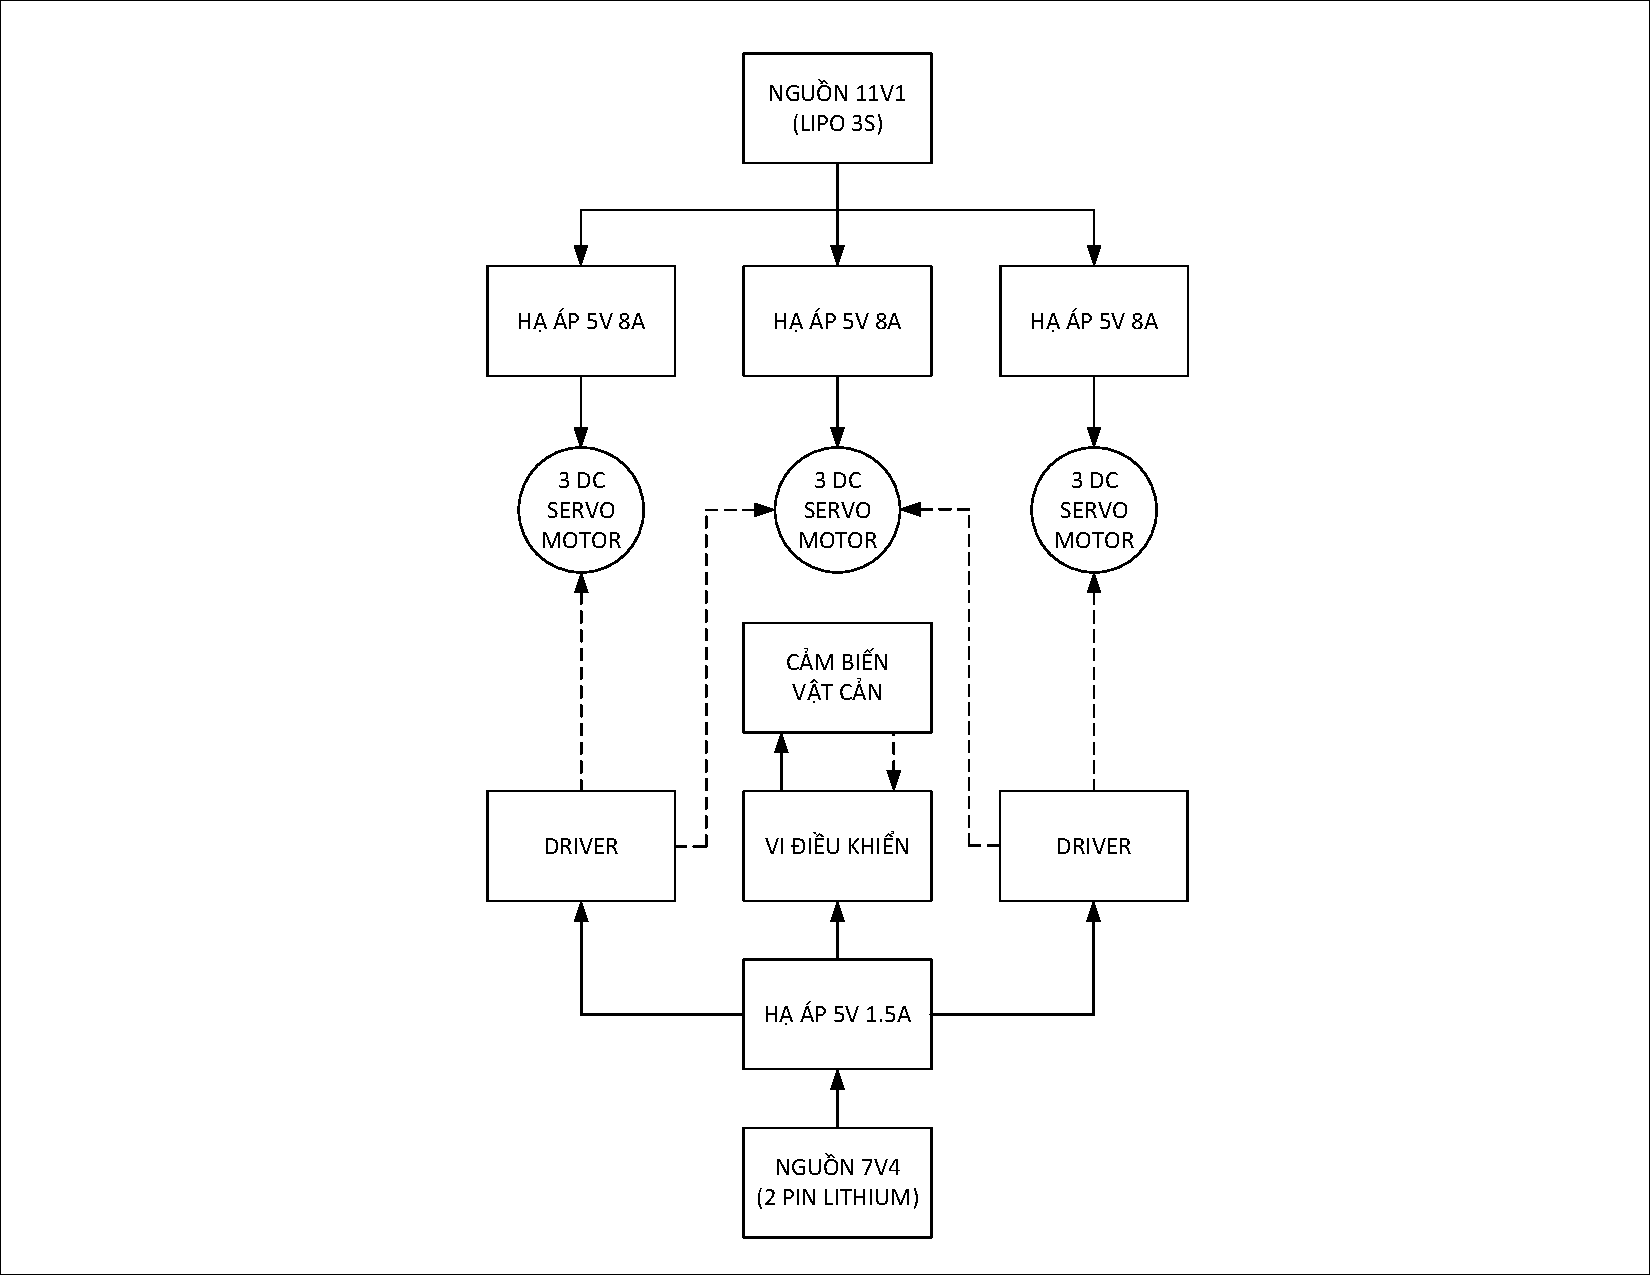
\includegraphics[width=1\textwidth, trim=0.1cm 0.1cm 0.1cm 0.1cm, clip]{pictures/ElectricalDiagram.pdf}                \caption{Sơ đồ khối hệ thống điện}
                \label{fig:block_diagram}
            \end{figure}
            
    \section{Thiết kế khái quát giải thuật điều khiển}

        \subsection{Kiến trúc phân tầng hệ điều khiển}

        \hspace{0.5cm} Hệ điều khiển robot nhện được tổ chức theo kiến trúc phân tầng gồm 4 lớp, từ giao tiếp người dùng xuống đến phần cứng servo:

        \begin{enumerate}
            \item \textbf{Lớp giao tiếp (Communication Layer):} Web app gửi lệnh JSON qua WebSocket đến ESP32 (WiFi SoftAP). Lớp này tiếp nhận lệnh \texttt{start}, \texttt{stop}, \texttt{set\_height}, \texttt{set\_gait}, \texttt{set\_foot}, đặt vào các biến trạng thái được bảo vệ bởi semaphore.
            \item \textbf{Lớp điều phối (Coordination Layer):} Vòng lặp chính trên FreeRTOS đọc trạng thái từ lớp giao tiếp, quản lý chuyển tiếp trạng thái Idle $\leftrightarrow$ Running, gọi gait controller theo chu kỳ, và tích hợp kết quả đo cảm biến SRF05 vào quyết định điều hướng.
            \item \textbf{Lớp giải thuật vận động (Motion Layer):} Gait controller tính toán vị trí đầu chân $(x,y,z)$ cho từng pha của dáng đi. Bộ giải động học nghịch (IK) chuyển đổi tọa độ Descartes sang góc khớp $(\theta_1, \theta_2, \theta_3)$ cho từng chân.
            \item \textbf{Lớp dẫn động (Actuation Layer):} Module PCA9685 nhận góc khớp, chuyển đổi sang độ rộng xung PWM và phát trực tiếp tới 18 servo.
        \end{enumerate}

        \subsection{Luồng điều khiển tổng quát}

        \hspace{0.5cm} Luồng điều khiển tổng quát của hệ thống diễn ra như sau:

        \begin{enumerate}
            \item Người dùng gửi lệnh \texttt{start} từ web app.
            \item ESP32 nhận lệnh qua WebSocket, đặt cờ \texttt{gait\_running = true}.
            \item Vòng lặp chính phát hiện chuyển tiếp Idle $\to$ Running, gọi \texttt{tripod\_init()} để đặt 6 chân vào tư thế khởi đầu.
            \item Mỗi vòng lặp: đo khoảng cách SRF05, cập nhật tham số điều hướng (trim), gọi \texttt{tripod\_step()}.
            \item \texttt{tripod\_step()} tính vị trí đầu chân cho từng pha, gọi IK, ghi góc servo ra PCA9685.
            \item Nếu SRF05 đo khoảng cách $< 20$ cm, đặt \texttt{trim\_y} để quay phải trong 6 bước tiếp theo.
            \item Nếu SRF05 đo khoảng cách $\geq 20$ cm, đặt \texttt{trim\_y} = 0 để đi thẳng.
            \item Khi nhận lệnh \texttt{set\_height}, cập nhật tham số chiều cao bước đi, áp dụng ngay cho bước tiếp theo.
            \item Khi nhận lệnh \texttt{stop}: hoàn thành bước hiện tại, đưa robot về tư thế đứng yên.
        \end{enumerate}

        \subsection{Phương án điều hướng}

        \hspace{0.5cm} Thay vì sử dụng bộ điều khiển kín (closed-loop) với cảm biến IMU, nhóm chọn phương án điều hướng mở (open-loop with trim): hướng di chuyển được điều chỉnh bằng cách lệch đối xứng tọa độ $y$ của các chân trong nhóm swing và stance. Tham số \texttt{trim\_y} (mm) dương tương ứng bẻ phải, âm tương ứng bẻ trái. Phương án này đơn giản, không cần IMU, nhưng không bù được nhiễu môi trường.

        Cảm biến SRF05 cung cấp phản hồi một chiều (khoảng cách phía trước), được tích hợp vào một state machine gồm hai trạng thái: \textbf{NORMAL} (đi thẳng hoặc lệch nhẹ) và \textbf{TURNING} (quay tại chỗ). Đây là dạng điều khiển phản xạ đơn giản (reactive control), không có bản đồ môi trường.

    \section{Thiết kế khái quát phần mềm}

        \subsection{Lựa chọn phương án giao diện điều khiển}

            \subsubsection{So sánh nền tảng giao diện}

            \hspace{0.5cm} Giao diện điều khiển robot cần đáp ứng các yêu cầu: hiển thị 3D thời gian thực, truyền lệnh hai chiều độ trễ thấp, không cần cài đặt phần mềm trên thiết bị người dùng và hoạt động được trên nhiều loại thiết bị (máy tính, điện thoại). Nhóm so sánh ba hướng tiếp cận phổ biến:

            \begin{table}[H]
            \centering
            \caption{So sánh các phương án nền tảng giao diện điều khiển}
            \label{tab:gui_options}
            \begin{tabular}{|>{\centering\arraybackslash}m{2.8cm}|>{\centering\arraybackslash}m{3.5cm}|>{\centering\arraybackslash}m{3.5cm}|>{\centering\arraybackslash}m{3.5cm}|}
            \hline
            \textbf{Tiêu chí} & \textbf{Windows Forms (.NET)} & \textbf{PyQt (Python)} & \textbf{Web App (trình duyệt)} \\
            \hline
            \textbf{Nền tảng} & Windows only & Windows, Linux, macOS & Mọi thiết bị có trình duyệt \\
            \hline
            \textbf{Cài đặt} & Cần cài .NET runtime & Cần cài Python + PyQt & Không cần cài đặt \\
            \hline
            \textbf{Đồ họa 3D} & Cần tích hợp OpenGL/DirectX & Cần tích hợp OpenGL & WebGL, Three.js sẵn có \\
            \hline
            \textbf{Truyền thông} & TCP socket, Serial & TCP socket, Serial & WebSocket, HTTP \\
            \hline
            \textbf{Cập nhật giao diện} & Phải build lại và cài lại & Phải build lại và cài lại & Chỉ cần cập nhật file trên ESP32 \\
            \hline
            \textbf{Hỗ trợ di động} & Không & Hạn chế & Có (responsive design) \\
            \hline
            \textbf{Độ phức tạp tích hợp} & Cao (cần driver riêng) & Trung bình & Thấp (WiFi SoftAP + trình duyệt) \\
            \hline
            \end{tabular}
            \end{table}

            \textbf{Kết luận:} Nhóm chọn \textbf{Web App} chạy trên trình duyệt. Phương án này không yêu cầu cài đặt phần mềm, hoạt động trên mọi thiết bị có WiFi và trình duyệt, tích hợp tự nhiên với WiFi SoftAP của ESP32, và có hệ sinh thái đồ họa 3D phong phú (WebGL/Three.js). Windows Forms bị loại do giới hạn nền tảng và yêu cầu cài đặt. PyQt bị loại do phức tạp khi triển khai trên nhiều thiết bị và hạn chế hỗ trợ di động.

            \subsubsection{So sánh phương án xây dựng web}

            \hspace{0.5cm} Sau khi chọn web app, nhóm so sánh hai hướng triển khai:

            \begin{table}[H]
            \centering
            \caption{So sánh HTML thuần và React SPA}
            \label{tab:web_framework}
            \begin{tabular}{|>{\centering\arraybackslash}m{3.5cm}|>{\centering\arraybackslash}m{5cm}|>{\centering\arraybackslash}m{5cm}|}
            \hline
            \textbf{Tiêu chí} & \textbf{HTML + JS thuần} & \textbf{React + Vite (SPA)} \\
            \hline
            \textbf{Quản lý trạng thái} & Thủ công (DOM manipulation) & Context API, useState, useEffect \\
            \hline
            \textbf{Cập nhật UI} & Phải tự cập nhật DOM & Tự động re-render khi state thay đổi \\
            \hline
            \textbf{Tái sử dụng code} & Khó, lặp lại nhiều & Component-based, dễ tái sử dụng \\
            \hline
            \textbf{Đồng bộ dữ liệu thực} & Phức tạp với nhiều nguồn dữ liệu & useEffect + Context đồng bộ tự động \\
            \hline
            \textbf{Hiệu năng animation} & requestAnimationFrame thủ công & Tích hợp tốt với RAF và Three.js \\
            \hline
            \textbf{Thư viện 3D} & Three.js (thuần) & React Three Fiber (wrapper React) \\
            \hline
            \textbf{Thời gian phát triển} & Nhanh ban đầu, khó mở rộng & Đầu tư ban đầu, dễ mở rộng \\
            \hline
            \end{tabular}
            \end{table}

            \textbf{Kết luận:} Nhóm chọn \textbf{React + Vite}. Với giao diện có nhiều thành phần đồng thời đọc cùng một nguồn dữ liệu WebSocket (viewer 3D, bảng góc, thanh trạng thái, settings panel), React Context API giúp đồng bộ trạng thái tự động mà không cần truyền props thủ công qua nhiều tầng. React Three Fiber cho phép tích hợp Three.js vào luồng React một cách tự nhiên.

        \subsection{Lựa chọn giao thức truyền thông}

            \subsubsection{So sánh giao thức truyền thông}

            \hspace{0.5cm} Giao tiếp giữa web app và ESP32 cần đáp ứng: độ trễ thấp (điều khiển realtime), hai chiều (lệnh điều khiển + phản hồi cảm biến), và dễ tích hợp trên ESP-IDF. Nhóm so sánh bốn giao thức phù hợp:

            \begin{table}[H]
            \centering
            \caption{So sánh các giao thức truyền thông web--ESP32}
            \label{tab:protocol_options}
            \begin{tabular}{|>{\centering\arraybackslash}m{2.5cm}|>{\centering\arraybackslash}m{2.5cm}|>{\centering\arraybackslash}m{2.5cm}|>{\centering\arraybackslash}m{2.5cm}|>{\centering\arraybackslash}m{2.5cm}|}
            \hline
            \textbf{Tiêu chí} & \textbf{HTTP Polling} & \textbf{HTTP SSE} & \textbf{WebSocket} & \textbf{MQTT} \\
            \hline
            \textbf{Mô hình} & Request--Response & Server push (1 chiều) & Full-duplex & Pub--Sub \\
            \hline
            \textbf{Độ trễ} & Cao (polling interval) & Trung bình & Thấp & Thấp \\
            \hline
            \textbf{Chiều truyền} & 1 chiều & 1 chiều (server→client) & 2 chiều & 2 chiều \\
            \hline
            \textbf{Overhead} & Header HTTP mỗi request & Thấp & Rất thấp (frame nhỏ) & Rất thấp \\
            \hline
            \textbf{Hỗ trợ trình duyệt} & Có & Có & Có & Cần thư viện JS \\
            \hline
            \textbf{Hỗ trợ ESP-IDF} & Có & Hạn chế & Có (esp\_http\_server) & Cần broker riêng \\
            \hline
            \textbf{Cần broker} & Không & Không & Không & Có \\
            \hline
            \end{tabular}
            \end{table}

            \textbf{Kết luận:} Nhóm chọn \textbf{WebSocket}. WebSocket là giao thức full-duplex duy nhất hỗ trợ sẵn trên trình duyệt, không cần broker bên ngoài, tích hợp trực tiếp vào \texttt{esp\_http\_server} của ESP-IDF, và có overhead frame rất thấp — phù hợp cho việc gửi lệnh điều khiển realtime và nhận liên tục dữ liệu cảm biến. HTTP Polling bị loại do độ trễ không ổn định theo chu kỳ polling. SSE bị loại do chỉ hỗ trợ một chiều server→client. MQTT bị loại do cần broker trung gian (không phù hợp với mô hình SoftAP độc lập).

            \subsubsection{Định dạng dữ liệu truyền}

            \hspace{0.5cm} Nhóm chọn \textbf{JSON văn bản} (thay vì binary protocol như MessagePack hay Protobuf) vì:
            \begin{itemize}
                \item Dễ đọc và debug trong quá trình phát triển (có thể dùng trực tiếp công cụ WebSocket test).
                \item ESP-IDF tích hợp sẵn thư viện \texttt{cJSON}, không cần thêm dependency.
                \item Kích thước bản tin nhỏ (dưới 100 byte/lệnh), overhead JSON không đáng kể so với yêu cầu bandwidth.
                \item JavaScript xử lý JSON gốc (\texttt{JSON.parse}/\texttt{JSON.stringify}), không cần schema thêm.
            \end{itemize}

        \subsection{Kiến trúc web app}

        \hspace{0.5cm} Web app được xây dựng theo kiến trúc \textbf{Single Page Application (SPA)} sử dụng React + Vite. Kiến trúc phân tầng gồm 3 lớp:

        \begin{enumerate}
            \item \textbf{Lớp giao tiếp (WsContext):} Quản lý kết nối WebSocket tới ESP32. Xử lý toàn bộ vòng đời kết nối (kết nối, ngắt kết nối, tái kết nối), gửi/nhận bản tin JSON, đo độ trễ (latency) qua cơ chế ping-pong, và phân phát dữ liệu nhận được (trạng thái robot, khoảng cách SRF05) tới các thành phần UI.
            \item \textbf{Lớp trạng thái robot (RobotContext):} Lưu trữ và quản lý toàn bộ trạng thái logic của robot trên client: chiều cao thân, tham số gait, offset servo, vị trí đầu chân, chế độ điều khiển. Đồng thời chạy vòng lặp hoạt hình (animation loop) mô phỏng dáng đi tripod trên trình duyệt khi không có dữ liệu thực từ robot.
            \item \textbf{Lớp giao diện (UI Components):} Gồm bốn thành phần chính: TopBar (kết nối, điều khiển chạy/dừng, hiển thị trạng thái), SettingsPanel (cài đặt offset, gait, pose mode), SpiderViewer (hiển thị 3D robot thời gian thực), AngleDisplay (bảng góc khớp số).
        \end{enumerate}

        \subsection{Giao thức giao tiếp WebSocket}

        \hspace{0.5cm} Giao tiếp giữa web app và firmware thực hiện qua WebSocket tại địa chỉ \texttt{ws://192.168.4.1/ws}. Tất cả bản tin sử dụng định dạng JSON. Luồng dữ liệu là hai chiều: web app gửi lệnh điều khiển, firmware phản hồi trạng thái và dữ liệu cảm biến.

        \subsection{Mô phỏng 3D trên trình duyệt}

        \hspace{0.5cm} Khi không kết nối hoặc không nhận được dữ liệu chân từ firmware, web app tự mô phỏng chuyển động tripod gait bằng vòng lặp \texttt{requestAnimationFrame} (RAF). Vị trí đầu chân được tính theo pha gait liên tục, sau đó chạy qua bộ IK (mirroring firmware) để ra góc khớp, rồi áp dụng forward kinematics để vẽ 3D. Khi kết nối và nhận dữ liệu thực từ firmware, viewer chuyển sang hiển thị trực tiếp góc khớp đo được.

